\documentclass{article}
\usepackage{cite, hyperref}

\title{contiBAIT: Improving Genome Assemblies Using Strand-seq Data}
\author{Kieran O'Neill, Mark Hills and Mike Gottlieb}

%\VignetteIndexEntry{flowBi}ngit 

\usepackage{Sweave}
\begin{document}
\Sconcordance{concordance:contiBAIT.tex:/data/ContiBAIT/vignettes/contiBAIT.Rnw:%
1 8 1 1 0 31 1 1 4 3 0 1 4 3 0 1 3 4 0 1 2 2 1 1 3 11 0 1 4 2 0 2 1 3 0 %
1 2 4 1 1 4 6 0 1 2 4 1 1 4 3 0 1 1 6 0 1 2 5 1 1 2 1 0 1 1 2 2 2 1 1 2 %
10 0 1 1 15 0 1 2 2 1 1 2 4 0 1 2 6 1}

\setkeys{Gin}{width=0.65\textwidth}
\setkeys{Gin}{height=0.65\textwidth}

\maketitle
\begin{center}
{\tt koneill@bcgsc.ca}
\end{center}

\textnormal{\normalfont}

\tableofcontents
\newpage

\section{Licensing}
Under the Two-Clause BSD License, you are free to use and redistribute this software.

\section{Introduction}
Strand-seq is a method for determining template strand inheritance in single cells.
When strand-seq data are collected for many cells from the same organism, spatially close genomic regions show similar patterns of template strand inheritance.
ContiBAIT allows users to leverage this property to carry out three tasks to improve draft genomes. Firstly, in assemblies made up entirely of contigs or scaffolds not yet assigned to chromosomes, these contigs can be clustered into chromosomes. Secondly, in assemblies wherein scaffolds have been assigned to chromosomes, but not yet placed on those chromosomes, those scaffolds can be placed in order relative to each other. Thirdly, for assemblies at the chromosome stage, where scaffolds are ordered and separated by many unbridged sequence gaps, the orientation of these sequence gaps can be found.  

All three of these tasks can be run in parallel, taking contig-stage assemblies and ordering all fragments first to chromosomes, then within chromosomes while simultaneously determining the relative orientation of each fragment.

\section{Input}
ContiBAIT requires input in BAM format. Multiple BAM files are required for analysis, so ContiBAIT specifically calls for users to identify a BAM directory in which to analyse. BAM files should be sorted prior to analysis.
To read in BAM files into ContiBAIT, create a strandFreqTable instance by calling strandSeqFreqTable() 

\begin{Schunk}
\begin{Sinput}
> # Read in BAM files. Path denotes location of the BAM files.
> # Returns a vector of file locations
> 
> library(contiBAIT)
> bamFileList <- list.files(
+ path=file.path(system.file(package='contiBAIT'), 'extdata'),
+ pattern=".bam$",
+ full.names=TRUE)
> # Create a strandFreqTable instance by calling strandSeqFreqTable  
> strandFrequencyList <- strandSeqFreqTable(bamFileList, 
+ qual=10, 
+ pairedEnd=FALSE)
\end{Sinput}
\end{Schunk}

This returns a list of two data.frames.  The first data.frame consists of a strand state frequency, calculated by taking the number of Watson (- strand) reads, subtracting the number of Crick (+ strand) reads, and dividing by the total number of reads.  These values range from -1 (entirely Watson reads) through to 1 (entirely Crick reads).  The second data.frame consists of the absolute number of reads covering the contig. This is used in thresholding the data, and in weighting the accuracy of calls in subsequent orderings.

\begin{Schunk}
\begin{Sinput}
> # Returned list consisting of two data.frames
> strandFrequencyList
\end{Sinput}
\begin{Soutput}
$strandTable
A matrix of strand frequencies for  76  contigs over  38  libraries.

$countTable
A matrix of read counts for  76  contigs over  38  libraries.
\end{Soutput}
\begin{Sinput}
> # Exclude strand state frequencies calculated from contigs with less than 10 reads
> 
> exampleStrandFreq <- strandFrequencyList[[1]]
> exampleReadCounts <- strandFrequencyList[[2]]
> exampleStrandFreq[which(exampleReadCounts < 10)] <- NA 
\end{Sinput}
\end{Schunk}

Additional information can be found on the help page for strandSeqFreqTable including all parameters.\\

The quality of the libraries, specifically whether the files being analysed appear to show the expected distributions of directional reads, can be assessed with plotWCdistributions.  In a diploid organism, there is an expectation that chromosomes will be derived from either two Watson homologues, one Watson and one Crick homologue, or two Crick homologues in a Mendelian 1:2:1 ratio.  In Strand-seq data, this will mean about 1/4 of the contigs will only have Watson reads mapping to them, and have a strand state frequency of -1, 1/4 of the contigs will only have Crick reads mapping to them, and have a strand state frequency of +1, and 1/2 of the contigs will have an approximately even mix of Watson and Crick reads (based on a binomial distribution of sampling).  plotWCDistribution generates boxplots for different strand state frequencies and models the expected distribution (blue line). The average called WW or CC contigs are shown in green, and should match closely with the expected distribution line.

\begin{Schunk}
\begin{Sinput}
> # Assess the quality of the libraries being analysed
> plotWCdistribution(exampleStrandFreq)
\end{Sinput}
\end{Schunk}
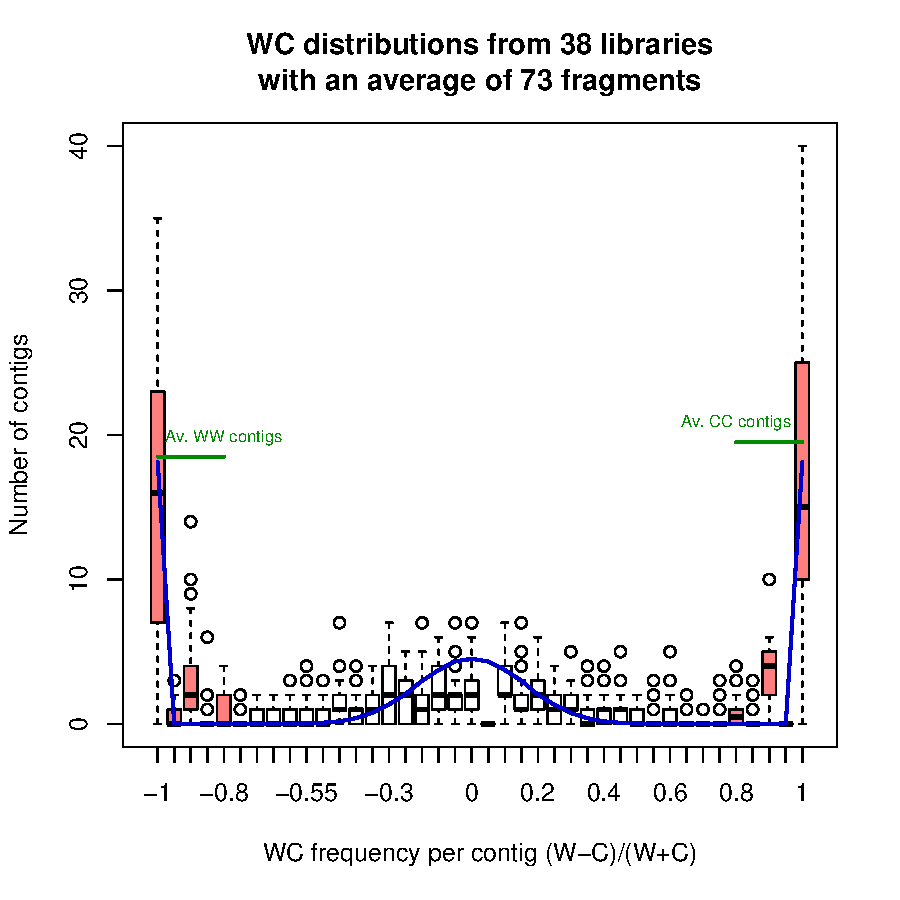
\includegraphics{contiBAIT-strandSeqFreqTableExamplec}

\section{Creating a strand state matrix}

The returned list of strandSeqFreqTable can be converted to a strand state matrix that makes a contig-wide call on the overall strand state based on the frequencies of Watson and Crick reads. The function removes BAM files that either contain too few reads to make accurate strand calls or are not strand-seq libraries (i.e. every contig contains approximately equal numbers of + and - reads). Conversely the function removes contigs that either contain too few reads, or always contain roughly equal numbers of + and - reads.  More details on the parameters can be found in the function documentation.  The function returns a similar data.frame to strandSeqFreqTable, but with the frequencies converted to strand calls: 1 is a homozygous Watson call (by default, a frequency less than -0.8, but this can be changed with the filterThreshold argument), 2 is a heterozygous call (a frequency between -0.8 and 0.8 by default) and 3 is a homozygous Crick call (by default, a frequency above 0.8).  These factors can then be used to cluster similar contigs together.\\

It is important to note that the relative directionality of any two fragments within an assembly is unknown. Contigs which belong on the same chromosome but are in different orientations will display as complete opposites; every library where one contig is homozygous Watson will have the other contig as homozygous Crick.  However, heterozygous contigs (where chromosomes inherited one Watson template and one Crick template), will not be mirrored, with one contig being "WC", while the other will be "CW".  As such, a data.frame without heterozygous calls is also generated to identify orientation issues.  
 

\begin{Schunk}
\begin{Sinput}
> # Convert strand frequencies to strand calls.
> 
> exampleStrandStateMatrix <- preprocessStrandTable(exampleStrandFreq, 
+ lowQualThreshold=0.8)
> exampleStrandStateMatrix[[1]]
\end{Sinput}
\begin{Soutput}
A strand state matrix for  76  contigs over  38  libraries.
\end{Soutput}
\end{Schunk}

\section{Clustering contigs into chromosomes}

TALK ABOUT clusterContigs

\begin{Schunk}
\begin{Sinput}
> exampleWCMatrix <- exampleStrandStateMatrix[[1]]
> exampleWWCCMatrix <- exampleStrandStateMatrix[[2]]
> clusteredContigs <- clusterContigs(exampleWWCCMatrix)
> LGOrientations <- reorientLinkageGroups(clusteredContigs, exampleWWCCMatrix)
> reorientedMatrix <- reorientStrandTable(exampleWCMatrix, linkageGroups=clusteredContigs, orientation=LGOrientations)
> exampleLGList <- mergeLinkageGroups(clusteredContigs,reorientedMatrix)
> exampleLGList
\end{Sinput}
\begin{Soutput}
A linkage group list containing  4  linkage groups.

  NumberOfContigs
1              19
2              19
3              19
4              19
\end{Soutput}
\begin{Sinput}
> exampleLGList[[1]]
\end{Sinput}
\begin{Soutput}
 [1] "chr1:160000000-161000000" "chr1:100000000-101000000"
 [3] "chr1:30000000-31000000"   "chr1:90000000-91000000"  
 [5] "chr1:240000000-241000000" "chr1:110000000-111000000"
 [7] "chr1:60000000-61000000"   "chr1:180000000-181000000"
 [9] "chr1:150000000-151000000" "chr1:1000000-2000000"    
[11] "chr1:80000000-81000000"   "chr1:50000000-51000000"  
[13] "chr1:20000000-21000000"   "chr1:70000000-71000000"  
[15] "chr1:120000000-121000000" "chr1:40000000-41000000"  
[17] "chr1:10000000-11000000"   "chr1:220000000-221000000"
[19] "chr1:200000000-201000000"
\end{Soutput}
\end{Schunk}


The clusterContigs function generates a list of linkage groups consisting of all the clustered contigs.  After reorientation and merging, all contigs within the linkage groups are highly similar, while the contigs between linkage groups are highly dissimilar.  The similarity between linkage groups can be visualized using plotLGDistances.

\begin{Schunk}
\begin{Sinput}
> plotLGDistances(exampleLGList, exampleWCMatrix)
\end{Sinput}
\end{Schunk}
\includegraphics{contiBAIT-clusterContigsExampleb}

While the similarity within linkage groups can be visualized using plotLinkageGroup (here, the first linkage group is used for creating this heatmap).

\begin{Schunk}
\begin{Sinput}
> plotLinkageGroup(exampleLGList[[1]], exampleWCMatrix)
\end{Sinput}
\end{Schunk}
\includegraphics{contiBAIT-clustercontigsExamplec}


\section{Ordering contigs within chromosomes}

greedy vs TSP

\begin{Schunk}
\begin{Sinput}
> contigOrder <- orderAllLinkageGroups(exampleLGList,
+ exampleWCMatrix,
+ exampleStrandFreq,
+ exampleReadCounts,
+ whichLG=1,
+ saveOrderedPDF=TRUE)
> contigOrder
\end{Sinput}
\begin{Soutput}
A data.frame of 1 LGs split into 15 sub-groups from 19 ordered fragments.

 LG1.1 LG1.10 LG1.11 LG1.12 LG1.13 LG1.14 LG1.15  LG1.2  LG1.3  LG1.4  LG1.5 
     1      1      3      1      1      1      1      2      1      1      1 
 LG1.6  LG1.7  LG1.8  LG1.9 
     2      1      1      1 
\end{Soutput}
\end{Schunk}
\includegraphics{contiBAIT-orderAllLinkageGroupsExample}

If the assembly is mostly complete and you wish to compare the actual location of the fragments against the output of orderAllLinkageGroups, contiBAIT has the built in plotContigOrder function 

\begin{Schunk}
\begin{Sinput}
> plotContigOrder(contigOrder$contig)
\end{Sinput}
\end{Schunk}
\includegraphics{contiBAIT-orderAllLinkageGroupsExampleb}


\section{Writing out to a BED file}
This file can be passed to bedtools along with the original (draft) reference genome to create a new FASTA file containing the assembled genome.


\section{creating a chromosome table instance}

The example data provided with the contiBAIT package is derived from sub-setted strand-Seq data split into 1 Mb fragments. To further analyse data, a chromosome table instance, representing the contig name and length can be generated with makeChrTable.  The resulting data.frame is similar to the header portion of a BAM file.  Using the addBED option will output a bed-format version of the same data.frame. 

\begin{Schunk}
\begin{Sinput}
> exampleChrTable <- makeChrTable(bamFileList[1]) 
> exampleChrTable
\end{Sinput}
\begin{Soutput}
A data.frame of 76 fragments from a  76 Mb genome.
                                          chr  length
chr1:1000000-2000000     chr1:1000000-2000000 1000000
chr1:10000000-11000000 chr1:10000000-11000000 1000000
chr1:20000000-21000000 chr1:20000000-21000000 1000000
chr1:30000000-31000000 chr1:30000000-31000000 1000000
chr1:40000000-41000000 chr1:40000000-41000000 1000000
chr1:50000000-51000000 chr1:50000000-51000000 1000000
...                                              chr  length
chr4:120000000-121000000 chr4:120000000-121000000 1000000
chr4:130000000-131000000 chr4:130000000-131000000 1000000
chr4:140000000-141000000 chr4:140000000-141000000 1000000
chr4:150000000-151000000 chr4:150000000-151000000 1000000
chr4:160000000-161000000 chr4:160000000-161000000 1000000
chr4:170000000-171000000 chr4:170000000-171000000 1000000
\end{Soutput}
\end{Schunk}

Furthermore, this chromosome table can be subdivided into smaller fragments. This is especially useful if there is a large degree of misorientations or chimerism in the data, but as the fragments get subdivided, the number of reads making strand state calls decreases.  Note the following divided chromosome table can be used with the filter argument in strandSeqFreqTable
to generate a sub-divided table.

\begin{Schunk}
\begin{Sinput}
> dividedChr <- divideMyChr(exampleChrTable, splitBy=50000)
> dividedChr
\end{Sinput}
\begin{Soutput}
A data.frame of 1596 fragments from a  76 Mb genome.
                                                    chr  start    end
chr1:1000000-2000000:0-50000       chr1:1000000-2000000      0  50000
chr1:1000000-2000000:50000-100000  chr1:1000000-2000000  50000 100000
chr1:1000000-2000000:100000-150000 chr1:1000000-2000000 100000 150000
chr1:1000000-2000000:150000-200000 chr1:1000000-2000000 150000 200000
chr1:1000000-2000000:200000-250000 chr1:1000000-2000000 200000 250000
chr1:1000000-2000000:250000-300000 chr1:1000000-2000000 250000 300000
...                                                              chr   start
chr4:170000000-171000000:750000-800000   chr4:170000000-171000000  750000
chr4:170000000-171000000:800000-850000   chr4:170000000-171000000  800000
chr4:170000000-171000000:850000-900000   chr4:170000000-171000000  850000
chr4:170000000-171000000:900000-950000   chr4:170000000-171000000  900000
chr4:170000000-171000000:950000-1000000  chr4:170000000-171000000  950000
chr4:170000000-171000000:1000000-1000000 chr4:170000000-171000000 1000000
                                             end
chr4:170000000-171000000:750000-800000    800000
chr4:170000000-171000000:800000-850000    850000
chr4:170000000-171000000:850000-900000    900000
chr4:170000000-171000000:900000-950000    950000
chr4:170000000-171000000:950000-1000000  1000000
chr4:170000000-171000000:1000000-1000000 1000000
\end{Soutput}
\end{Schunk}

Or for splitting by sites of state change (IN DEVELOP)

With a chromosome table instance, comparisons can be made between the portion of contigs that are included in the analysis verses those that are excluded based on either poor coverage or non-Strand-seq patterning.  The code below generates a box plot of contig sizes that are included in the analysis. Note, since sample data are uniform 1 Mb framgents, the box plot does not deviate from the median.

\begin{Schunk}
\begin{Sinput}
> makeBoxPlot(exampleChrTable, exampleLGList)
\end{Sinput}
\end{Schunk}
\includegraphics{contiBAIT-makeChrTableExamplec}



\begin{Schunk}
\begin{Sinput}
> barplotLinkageGroupCalls(exampleLGList, exampleChrTable)
\end{Sinput}
\end{Schunk}
\includegraphics{contiBAIT-makeChrTableExampled}



\end{document}
